% This file was created with tikzplotlib v0.10.1.
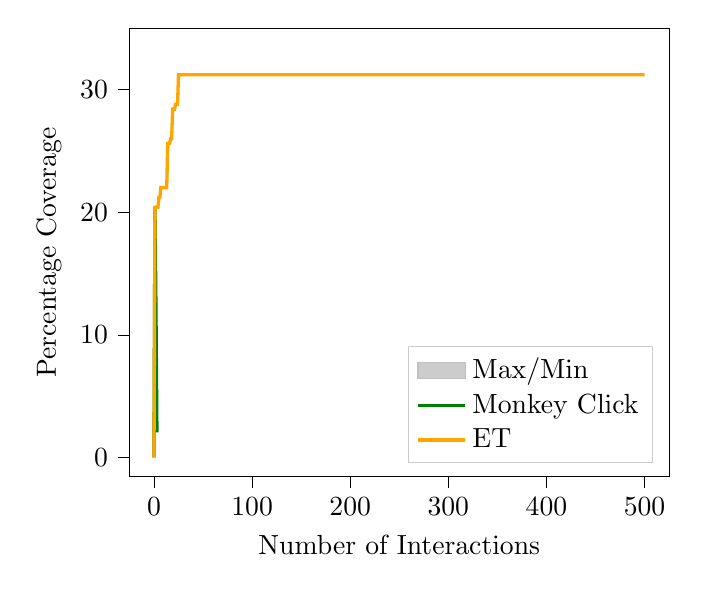
\begin{tikzpicture}

\definecolor{darkgray176}{RGB}{176,176,176}
\definecolor{green}{RGB}{0,128,0}
\definecolor{lightgray204}{RGB}{204,204,204}
\definecolor{orange}{RGB}{255,165,0}
\definecolor{silver}{RGB}{192,192,192}

\begin{axis}[
legend cell align={left},
legend style={
  fill opacity=0.8,
  draw opacity=1,
  text opacity=1,
  at={(0.97,0.03)},
  anchor=south east,
  draw=lightgray204
},
tick align=outside,
tick pos=left,
x grid style={darkgray176},
xlabel={Number of Interactions},
xmin=-25, xmax=525,
xtick style={color=black},
y grid style={darkgray176},
ylabel={Percentage Coverage},
ymin=-1.56, ymax=35,
ytick style={color=black}
]
\path [draw=silver, fill=silver]
(axis cs:0,0)
--(axis cs:0,0)
--(axis cs:1,20.4)
--(axis cs:2,20.4)
--(axis cs:3,20.4)
--(axis cs:3,20.4)
--(axis cs:3,20.4)
--(axis cs:2,20.4)
--(axis cs:1,20.4)
--(axis cs:0,0)
--cycle;
\addlegendimage{area legend, draw=silver, fill=silver}
\addlegendentry{Max/Min}

\addplot [very thick, green]
table {%
0 0
1 20.4
2 12.24
3 2.04
};
\addlegendentry{Monkey Click}
\addplot [very thick, orange]
table {%
0 0
1 20.4
2 20.4
3 20.4
4 20.4
5 21.2
6 21.2
7 22
8 22
9 22
10 22
11 22
12 22
13 22
14 25.6
15 25.6
16 25.6
17 26
18 26
19 28.4
20 28.4
21 28.4
22 28.8
23 28.8
24 28.8
25 31.2
26 31.2
27 31.2
28 31.2
29 31.2
30 31.2
31 31.2
32 31.2
33 31.2
34 31.2
35 31.2
36 31.2
37 31.2
38 31.2
39 31.2
40 31.2
41 31.2
42 31.2
43 31.2
44 31.2
45 31.2
46 31.2
47 31.2
48 31.2
49 31.2
50 31.2
51 31.2
52 31.2
53 31.2
54 31.2
55 31.2
56 31.2
57 31.2
58 31.2
59 31.2
60 31.2
61 31.2
62 31.2
63 31.2
64 31.2
65 31.2
66 31.2
67 31.2
68 31.2
69 31.2
70 31.2
71 31.2
72 31.2
73 31.2
74 31.2
75 31.2
76 31.2
77 31.2
78 31.2
79 31.2
80 31.2
81 31.2
82 31.2
83 31.2
84 31.2
85 31.2
86 31.2
87 31.2
88 31.2
89 31.2
90 31.2
91 31.2
92 31.2
93 31.2
94 31.2
95 31.2
96 31.2
97 31.2
98 31.2
99 31.2
100 31.2
101 31.2
102 31.2
103 31.2
104 31.2
105 31.2
106 31.2
107 31.2
108 31.2
109 31.2
110 31.2
111 31.2
112 31.2
113 31.2
114 31.2
115 31.2
116 31.2
117 31.2
118 31.2
119 31.2
120 31.2
121 31.2
122 31.2
123 31.2
124 31.2
125 31.2
126 31.2
127 31.2
128 31.2
129 31.2
130 31.2
131 31.2
132 31.2
133 31.2
134 31.2
135 31.2
136 31.2
137 31.2
138 31.2
139 31.2
140 31.2
141 31.2
142 31.2
143 31.2
144 31.2
145 31.2
146 31.2
147 31.2
148 31.2
149 31.2
150 31.2
151 31.2
152 31.2
153 31.2
154 31.2
155 31.2
156 31.2
157 31.2
158 31.2
159 31.2
160 31.2
161 31.2
162 31.2
163 31.2
164 31.2
165 31.2
166 31.2
167 31.2
168 31.2
169 31.2
170 31.2
171 31.2
172 31.2
173 31.2
174 31.2
175 31.2
176 31.2
177 31.2
178 31.2
179 31.2
180 31.2
181 31.2
182 31.2
183 31.2
184 31.2
185 31.2
186 31.2
187 31.2
188 31.2
189 31.2
190 31.2
191 31.2
192 31.2
193 31.2
194 31.2
195 31.2
196 31.2
197 31.2
198 31.2
199 31.2
200 31.2
201 31.2
202 31.2
203 31.2
204 31.2
205 31.2
206 31.2
207 31.2
208 31.2
209 31.2
210 31.2
211 31.2
212 31.2
213 31.2
214 31.2
215 31.2
216 31.2
217 31.2
218 31.2
219 31.2
220 31.2
221 31.2
222 31.2
223 31.2
224 31.2
225 31.2
226 31.2
227 31.2
228 31.2
229 31.2
230 31.2
231 31.2
232 31.2
233 31.2
234 31.2
235 31.2
236 31.2
237 31.2
238 31.2
239 31.2
240 31.2
241 31.2
242 31.2
243 31.2
244 31.2
245 31.2
246 31.2
247 31.2
248 31.2
249 31.2
250 31.2
251 31.2
252 31.2
253 31.2
254 31.2
255 31.2
256 31.2
257 31.2
258 31.2
259 31.2
260 31.2
261 31.2
262 31.2
263 31.2
264 31.2
265 31.2
266 31.2
267 31.2
268 31.2
269 31.2
270 31.2
271 31.2
272 31.2
273 31.2
274 31.2
275 31.2
276 31.2
277 31.2
278 31.2
279 31.2
280 31.2
281 31.2
282 31.2
283 31.2
284 31.2
285 31.2
286 31.2
287 31.2
288 31.2
289 31.2
290 31.2
291 31.2
292 31.2
293 31.2
294 31.2
295 31.2
296 31.2
297 31.2
298 31.2
299 31.2
300 31.2
301 31.2
302 31.2
303 31.2
304 31.2
305 31.2
306 31.2
307 31.2
308 31.2
309 31.2
310 31.2
311 31.2
312 31.2
313 31.2
314 31.2
315 31.2
316 31.2
317 31.2
318 31.2
319 31.2
320 31.2
321 31.2
322 31.2
323 31.2
324 31.2
325 31.2
326 31.2
327 31.2
328 31.2
329 31.2
330 31.2
331 31.2
332 31.2
333 31.2
334 31.2
335 31.2
336 31.2
337 31.2
338 31.2
339 31.2
340 31.2
341 31.2
342 31.2
343 31.2
344 31.2
345 31.2
346 31.2
347 31.2
348 31.2
349 31.2
350 31.2
351 31.2
352 31.2
353 31.2
354 31.2
355 31.2
356 31.2
357 31.2
358 31.2
359 31.2
360 31.2
361 31.2
362 31.2
363 31.2
364 31.2
365 31.2
366 31.2
367 31.2
368 31.2
369 31.2
370 31.2
371 31.2
372 31.2
373 31.2
374 31.2
375 31.2
376 31.2
377 31.2
378 31.2
379 31.2
380 31.2
381 31.2
382 31.2
383 31.2
384 31.2
385 31.2
386 31.2
387 31.2
388 31.2
389 31.2
390 31.2
391 31.2
392 31.2
393 31.2
394 31.2
395 31.2
396 31.2
397 31.2
398 31.2
399 31.2
400 31.2
401 31.2
402 31.2
403 31.2
404 31.2
405 31.2
406 31.2
407 31.2
408 31.2
409 31.2
410 31.2
411 31.2
412 31.2
413 31.2
414 31.2
415 31.2
416 31.2
417 31.2
418 31.2
419 31.2
420 31.2
421 31.2
422 31.2
423 31.2
424 31.2
425 31.2
426 31.2
427 31.2
428 31.2
429 31.2
430 31.2
431 31.2
432 31.2
433 31.2
434 31.2
435 31.2
436 31.2
437 31.2
438 31.2
439 31.2
440 31.2
441 31.2
442 31.2
443 31.2
444 31.2
445 31.2
446 31.2
447 31.2
448 31.2
449 31.2
450 31.2
451 31.2
452 31.2
453 31.2
454 31.2
455 31.2
456 31.2
457 31.2
458 31.2
459 31.2
460 31.2
461 31.2
462 31.2
463 31.2
464 31.2
465 31.2
466 31.2
467 31.2
468 31.2
469 31.2
470 31.2
471 31.2
472 31.2
473 31.2
474 31.2
475 31.2
476 31.2
477 31.2
478 31.2
479 31.2
480 31.2
481 31.2
482 31.2
483 31.2
484 31.2
485 31.2
486 31.2
487 31.2
488 31.2
489 31.2
490 31.2
491 31.2
492 31.2
493 31.2
494 31.2
495 31.2
496 31.2
497 31.2
498 31.2
499 31.2
500 31.2
};
\addlegendentry{ET}
\end{axis}

\end{tikzpicture}
